\chapter{Wykład 9. Zarządzanie czasem w projekcie informatycznym}

\section{SPP uwzglęniający plan kont kosztowych projektu}
% strona 34

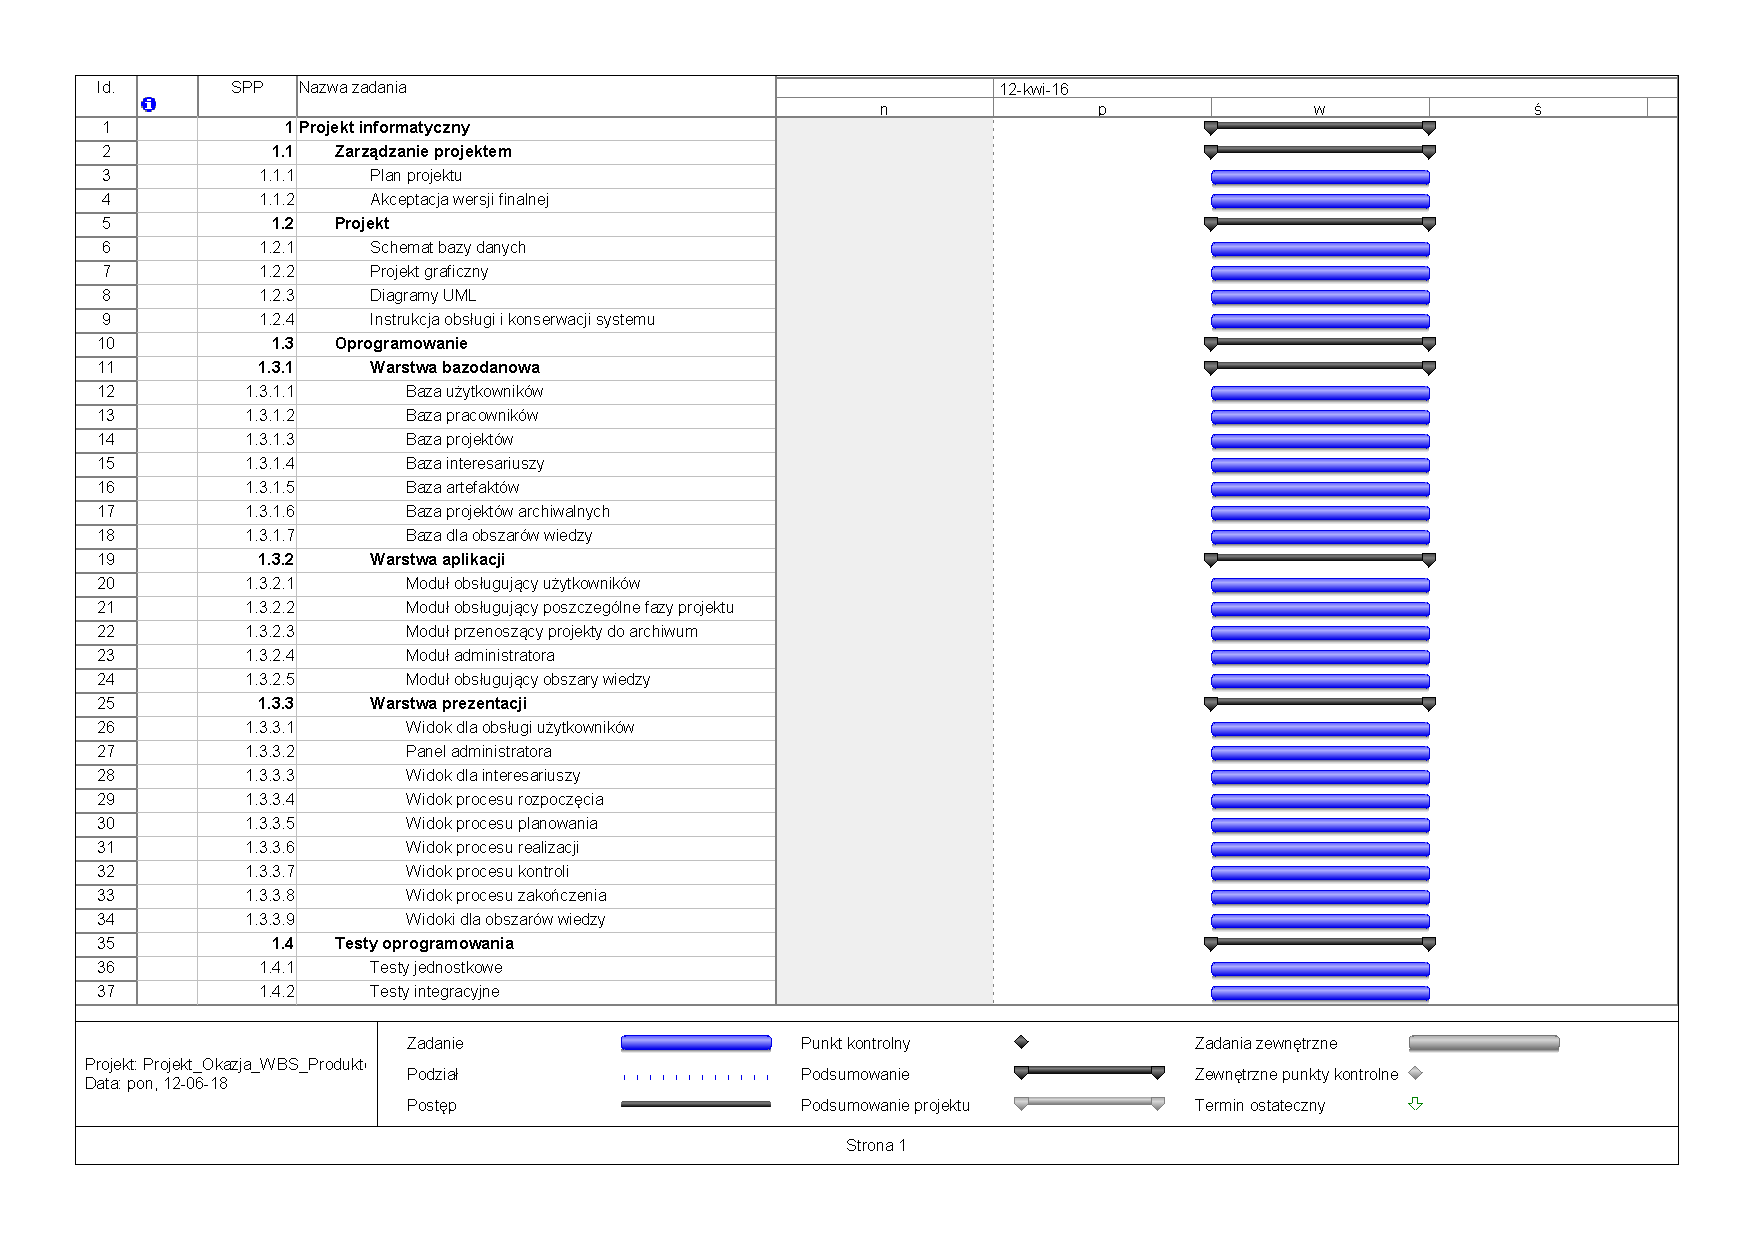
\includepdf[nup=1x2,pages=-]{diagramSPP.pdf}

% ===========================================================================

\section{Harmonogram w MS Project}
% strona 35

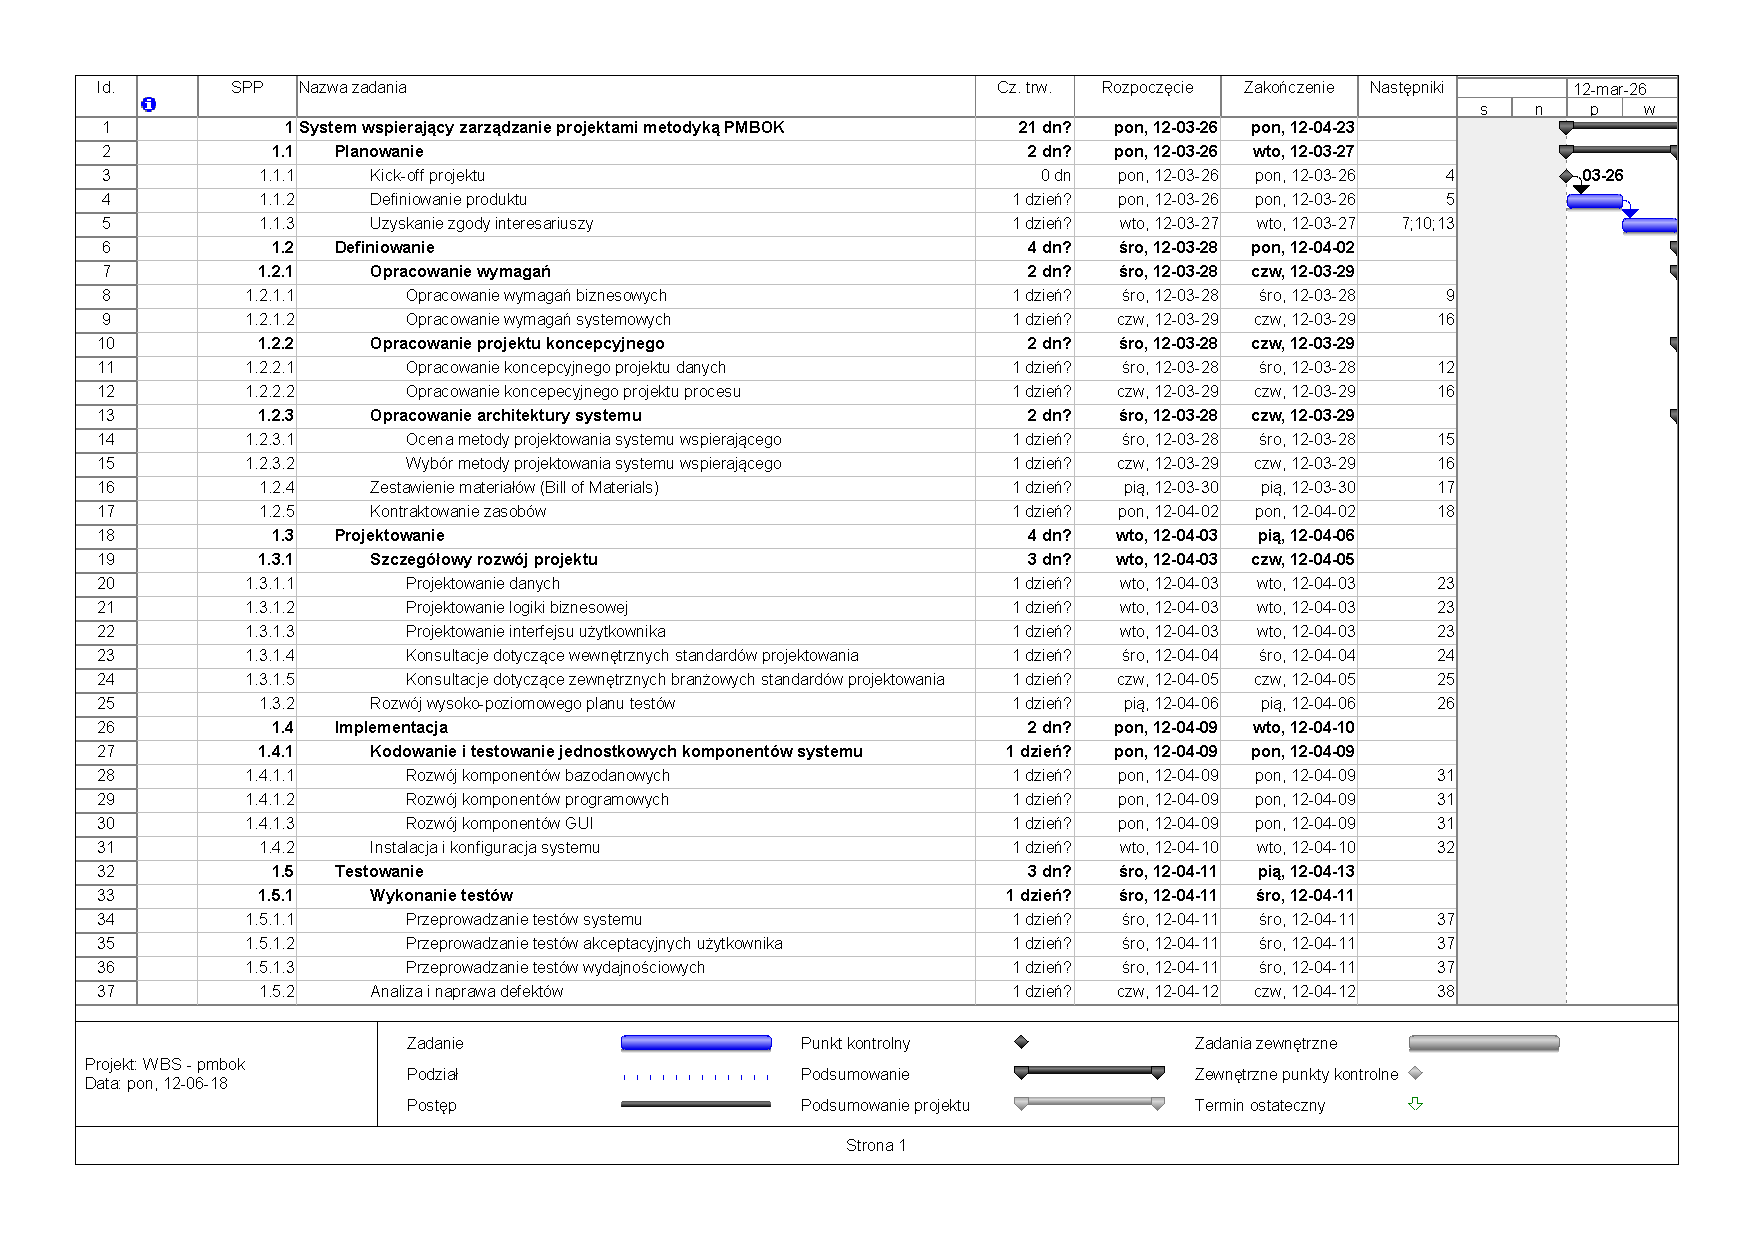
\includepdf[nup=2x2,pages=-,landscape=true,column=true]{harmonogramWBS.pdf}

% ===========================================================================

\section{Struktura RBS projektu}
% strona 45

\begin{figure}[htb]
\begin{center}
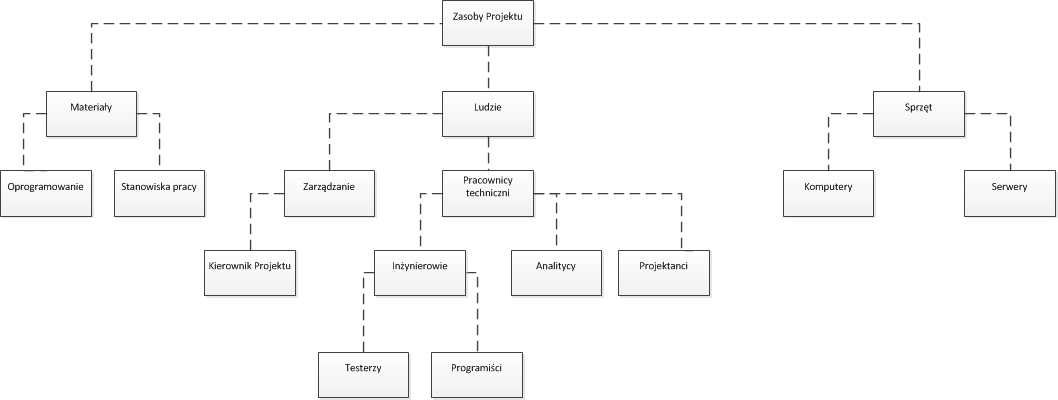
\includegraphics[width=\textwidth]{RBS.png}
\caption[RBS]{RBS}
\label{rysunekProces}
\end{center}
\end{figure}

% ===========================================================================

\section{Harmonogram z uwzględnieniem zasobów}
% strona 59

\begin{figure}[hbt]
\centering
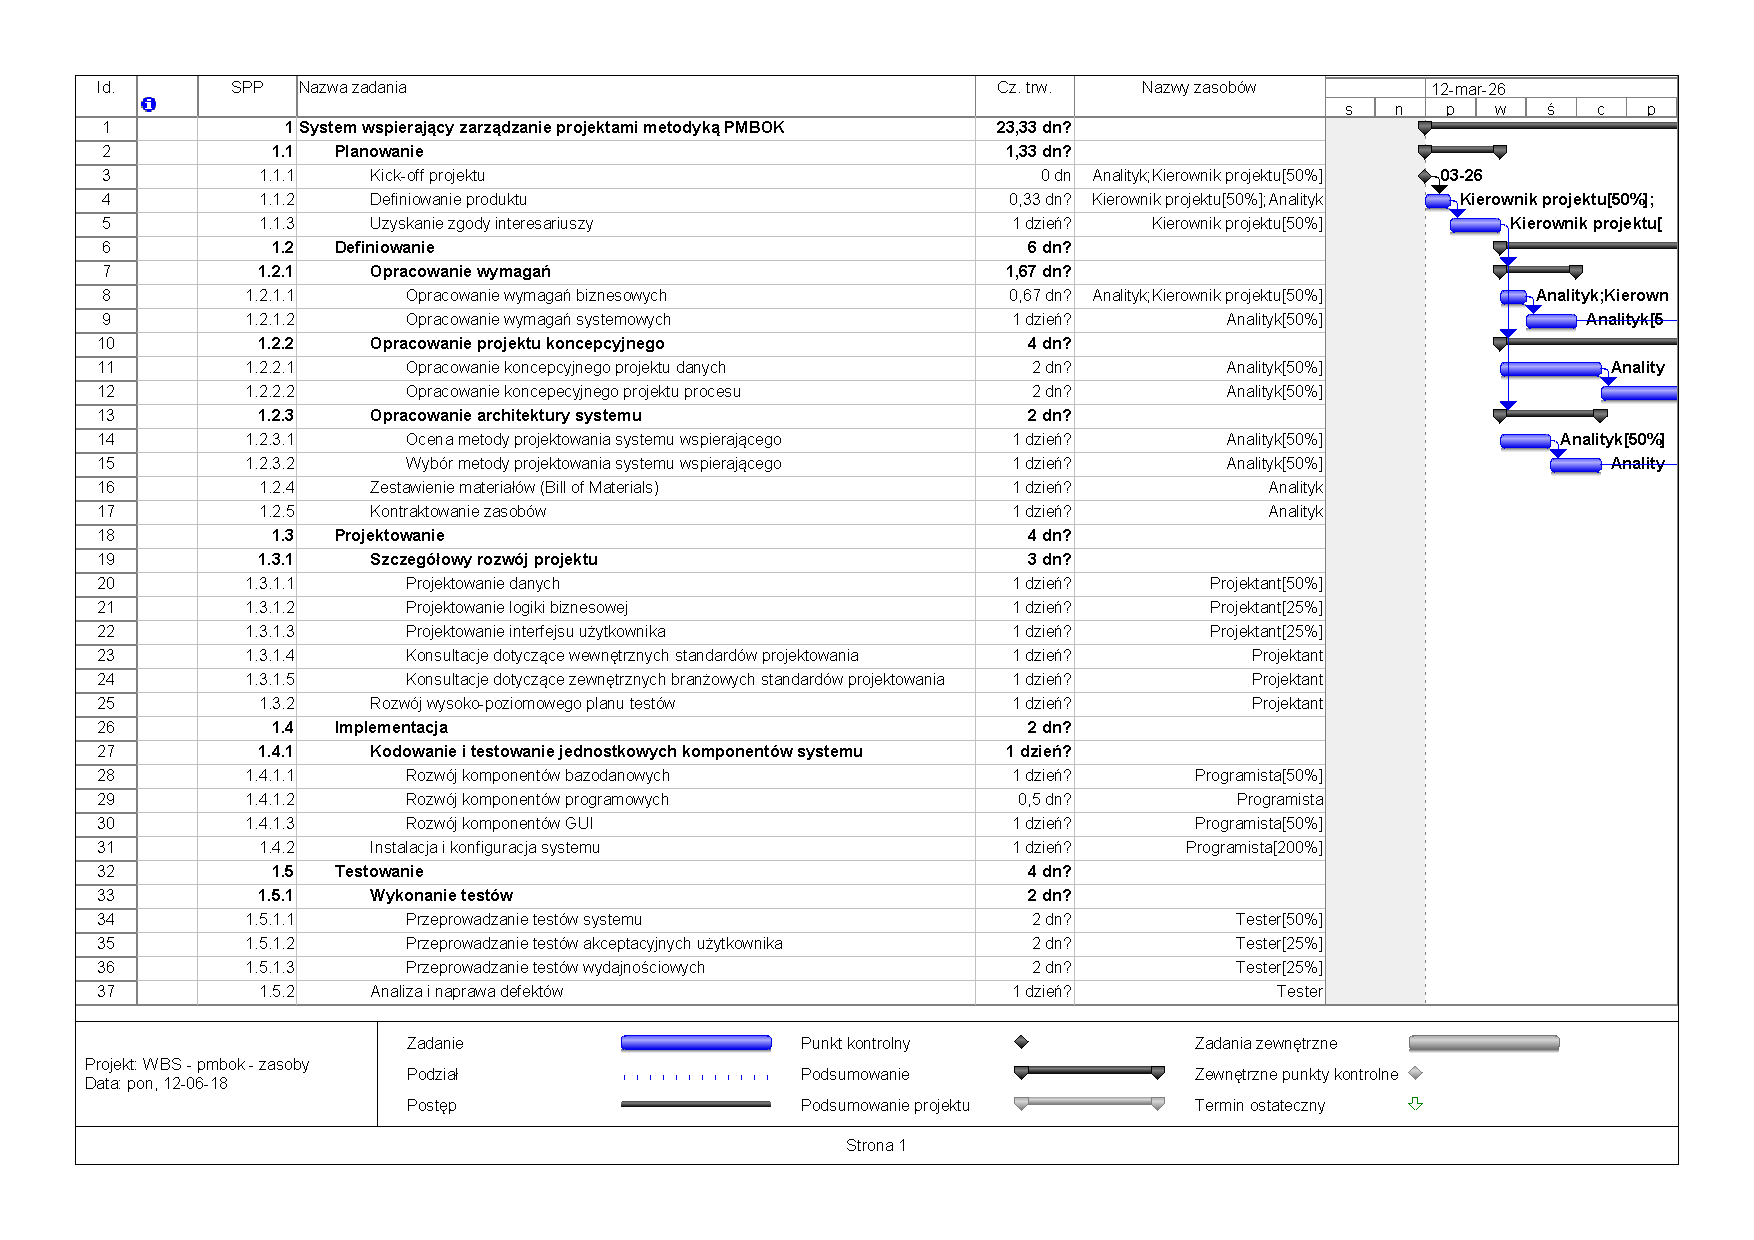
\includegraphics[width=1.1\textwidth]{zasobyWBS.pdf}
\caption{Harmonogram z zasobami}
\label{fig:zasobyWBS}
\end{figure}


